% !TeX root = ../thuthesis-example.tex

\chapter{卷积神经网络的分层抽象特性和遗忘方法}
上一章阐述了遗忘学习的研究现状和面临的主要挑战。本章的主要内容是介绍卷积神经网络的一个重要特性,即分层抽象特性。为了让读者能够更好地理解卷积神经网络的分层抽象特性,我们将首先介绍卷积神经网络的工作原理以及其中较为深层的设计思想。接下来我们会正式定义机器学习遗忘的概念,再介绍基于卷积神经网络分层抽象特性的遗忘思想。最后将介绍评价遗忘的性能指标。

\section{卷积神经网络的介绍}

\subsection{卷积神经网络的结构}
\paragraph{}首先,我们看卷积神经网络的网络结构,大致了解卷积神经网络的框架。卷积神经网络和多层感知机的神经网络很类似,它们都可以通过像堆积木一样来组装构建。然而,卷积神经网络里和多层感知机不同的是出现了Convolution 层(通常称为卷积层)和Pooling 层(通常称为池化层)。
\paragraph{}下一小节会详细介绍卷积层与池化层,在这我们首先看如何将各层组织起来构建卷积神经网络。基于多层感知机的神经网络中,相邻层的各个神经元之间都有连接,这样的结构被称为fully-connected(通常称为全连接)。Pytorch工具中已经实现了全连接层。如果使用全连接层来搭建网络,我们可以通过如图\ref{fig:chapter3_3}所示的神经网络结构实现一个五层的简单神经网络。
如图\ref{fig:chapter3_3}所示,在使用全连接层搭建的神经网络中,全连接层后面直接跟着激活函数ReLU(或者Sigmoid)。这里使用了4 层全连接和ReLU的组合,接着的第5层是全连接层,最后一层则是Softmax层,输出最终的预测结果。
\begin{figure}
    \centering
    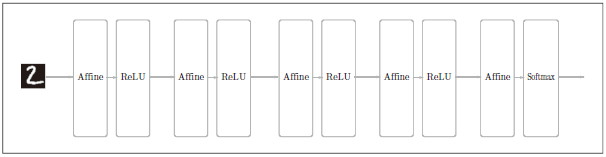
\includegraphics[width=0.9\linewidth]{chapter3_3.png}
    \caption{全连接网络结构示意图}
    \label{fig:chapter3_3}
\end{figure}
如图\ref{fig:chapter3_2}所示,这就是一个卷积神经网络的例子。
\begin{figure}
    \centering
    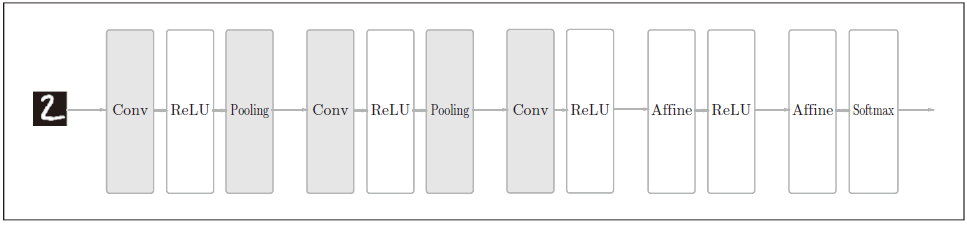
\includegraphics[width=0.9\linewidth]{chapter3_2.png}
    \caption{卷积神经网络结构示意图}
    \label{fig:chapter3_2}
\end{figure}
如图\ref{fig:chapter3_2}所示,卷积神经网络中增加了卷积层和池化层。卷积神经网络的单个层连接的顺序是卷积层,激活函数层和池化层,其中池化层有时可以省略。这样的组合方式可以被理解为前面的全连接层和激活函数层组合连接被替换成了卷积层,激活函数层和池化层的连接。另外,在如图所示的卷积神经网络中,靠近后面的输出层中使用了全连接层和激活函数层ReLU组合。然后,最终的输出层中则使用了全连接层和Softmax的组合。这样的搭配一般都是卷积神经网络中较为常见的搭配结构。
\subsection{卷积神经网络的原理}
\paragraph{}在全连接的神经网络中,各个层次都是通过全连接层来组织起来的。在全连接的层次中,各个神经元都是连接在一起的,全连接的网络的输出数量是可以任意指定的,没有数量上的限制。
\paragraph{}这样的结构会带来一定的问题,那就是数据的形状特征没有被充分地利用起来。用图片来举例,神经网络输入图片时,图片数据的格式一般是长、宽和高。长和宽代表图片像素点的长度和宽度,高代表图片采样通道的宽度。然而,这样的数据结构输入到全连接层搭建的神经网络中时,就会被拉长为一维的数据。举例说明,MNIST的数据集中一张图片的长是28个像素点,宽是28个像素点,高度是1个通道(图片用黑白表示)。这样的形状输入到全连接的网络中前会被展开成一列,就是784个数据点输入到网络中。按照常识可以知道,图片一般是三维的形状。
\paragraph{}这样的形状结构中包含重要的空间位置关系信息。比如通道与通道之间的关联信息,空间上相互距离比较接近的像素点一般具有相似的值,距离比较远的像素点一般没有关联,因此三维形状的数据中可能会蕴藏很多可以挖掘的特征模式。全是全连接层的神经网络就会把数据拉长成一维数据,从而没有充分利用图片中的空间位置信息。
\paragraph{}卷积神经网络就不会这样,图片输入到网络中就是以三维数据的格式输入,一个卷积层处理好数据以后,让然会以三维的格式输入到下一个卷积层中。所以,卷积神经网络对于理解图像这样带有空间位置信息的数据是很有优势的。
\subsubsection{卷积层}

\subsubsection{池化层}

\section{卷积神经网络的分层抽象特性}
\subsection{人类视觉信息处理原理}
\paragraph{}在讲卷积神经网络的分层抽象特性之前我们看看人类视觉是如何处理外界输入的。1981年诺贝尔生物学奖颁发给来自哈佛大学的大卫休伯尔(David Hubel)和维泽尔(Torsten Weisel),以表彰他们在人类视觉通路原理方面的研究对人类发展做出的巨大贡献。在他们的研究中指出人类视觉处理是分层次的。人类视觉的输入是视网膜,视网膜将外界环境进入眼睛的光信号转换为可以在神经元间传递的电信号。下一层的神经元激活的特征是具有选择性,即某些神经元只接受某个方向上移动的信号,这称为朝向选择性;而某些神经元只接受具有某种颜色的信号,这称为颜色选择性。具有选择性的这些神经细胞又组成了视觉神经系统的一层, 这一层将视网膜输入的信息进行了第一次抽象,最终输出的是一些具有某种特征的信号给下一层,比如具有某种朝向的信号和颜色信号。下一层根据上一层的输入再进行一次抽象,通过将朝向信息和颜色信息组合起来就能判别出外界输入的形状信息。有了形状信息之后,比较高层的神经细胞经过几次类似的抽象之后就能够根据这些信息生成外界输入信号的较为整体的信息。我们以人脸识别为例来说明一下这个过程,如图\ref{fig:chapter3_1}所示。
\begin{figure}
    \centering
    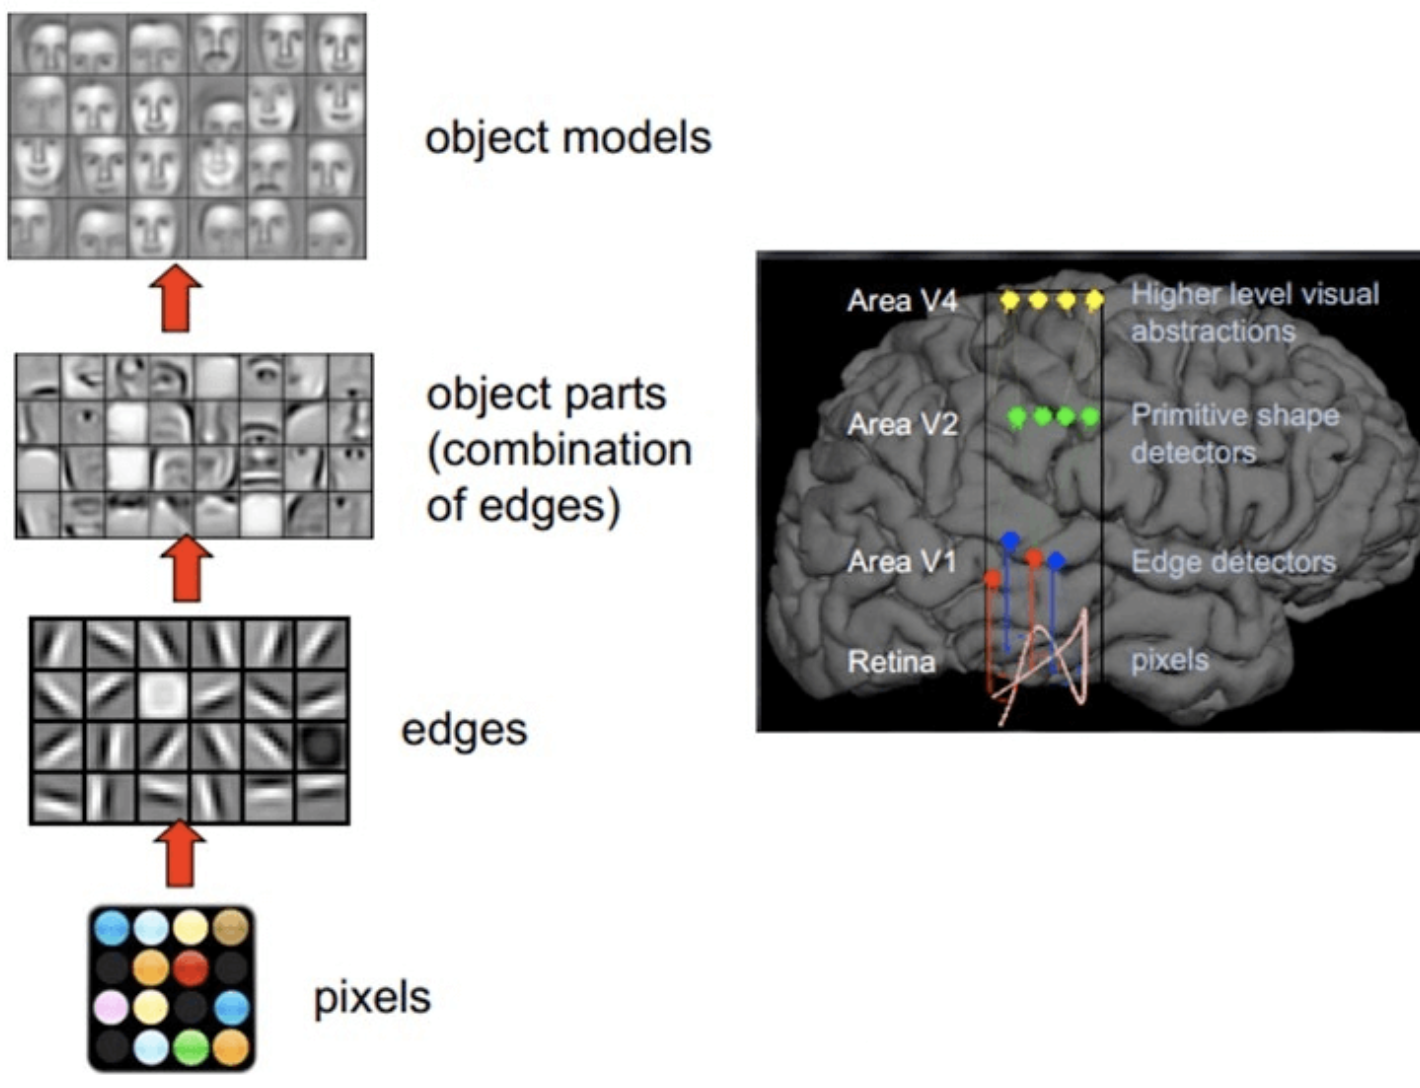
\includegraphics[width=0.9\linewidth]{chapter3_1.png}
    \caption{人类视觉处理信息流程示意图}
    \label{fig:chapter3_1}
\end{figure}

\subsection{卷积神经网络的分层抽象特性}

\section{基于卷积神经网络的遗忘方法}

\subsection{确定分层}

\subsection{重置并冻结参数}

\subsection{训练网络}

\section{遗忘效果的衡量指标}

\subsection{遗忘集、保留集和测试集准确率}

\subsection{收敛时间}

\subsection{激活距离}

\subsection{成员推断攻击成功率}

\section{本章小结}

